\documentclass[10pt,a4paper]{article}
\usepackage[margin=2.25cm,top=2.45cm,bottom=2.4cm]{geometry}
\usepackage[T1]{fontenc}
\usepackage{lmodern,microtype,booktabs,tabularx,array,graphicx,xcolor}
\usepackage{enumitem,caption,fancyhdr,xurl,float}
\usepackage[unicode,colorlinks=true,urlcolor=blue!65!black,linkcolor=black]{hyperref}
\graphicspath{{../analysis/figures/}}
\definecolor{ink}{HTML}{202A32}
\definecolor{navy}{HTML}{173E56}
\definecolor{muted}{HTML}{586974}
\definecolor{rule}{HTML}{CED8DD}
\color{ink}
\setlength{\parindent}{0pt}
\setlength{\parskip}{0.35em}
\setlength{\emergencystretch}{2em}
\renewcommand{\arraystretch}{1.17}
\captionsetup{font=small,labelfont=bf}
\setlist[itemize]{leftmargin=1.25em,itemsep=0.1em,topsep=0.15em}
\pagestyle{fancy}
\setlength{\headheight}{22pt}
\fancyhf{}
\fancyhead[L]{\footnotesize\color{muted} IIB423T-1 \quad / \quad Workshop 1}
\fancyhead[R]{\footnotesize\color{muted} Medina \& Castillo}
\fancyfoot[R]{\footnotesize\color{muted}\thepage}
\renewcommand{\headrulewidth}{0.35pt}
\renewcommand{\headrule}{\hbox to\headwidth{\color{rule}\leaders\hrule height \headrulewidth\hfill}}
\newcommand{\sectionhead}[1]{\vspace{0.34em}{\large\bfseries\color{navy}#1}\par\vspace{0.08em}}
\newcommand{\subhead}[1]{\vspace{0.18em}{\bfseries #1}\par}
\newcommand{\source}[1]{\textsuperscript{[#1]}}

\begin{document}
\thispagestyle{empty}
{\small\bfseries\color{navy} BUSINESS INTELLIGENCE \hspace{0.7em} / \hspace{0.7em} WORKSHOP 1}\par
\vspace{0.6em}
{\LARGE\bfseries Two directions for an online retail case}\par
\vspace{0.35em}
{\large Customer concentration and cancellation records}\par
\vspace{0.55em}
{\color{muted} Mois\'{e}s Medina \quad and \quad Ignacia Castillo \hfill 25 September 2026}\par
\vspace{0.6em}{\color{rule}\hrule height 0.65pt}\vspace{0.55em}

\textbf{Provisional choice.} We would take \emph{customer concentration in recorded purchase value} into C1. It has a measurable outcome and a sharper question than the predictable monthly peak: how dependent is observed value on a small group of customers? Cancellation records offer a distinct operations question, but the file cannot link a cancellation to its original purchase. We keep both candidates open for instructor feedback.

\sectionhead{1\quad Source, scope and observation unit}
We use Daqing Chen's \emph{Online Retail} dataset from UCI (DOI 10.24432/C5BW33), licensed CC BY 4.0. UCI describes 541,909 transactions from a UK-based online gift retailer, dated 1 December 2010 to 9 December 2011. Its dictionary defines \texttt{InvoiceNo}, \texttt{StockCode}, product description, quantity, invoice date, sterling unit price, customer ID and customer country; an invoice beginning with ``C'' indicates a cancellation.\source{1} In our analysis, one row is a recorded \emph{invoice line}, while \texttt{InvoiceNo} identifies the broader invoice. Neither a line nor an invoice is necessarily a unique customer.

To avoid comparing a full month with only nine days, we kept \textbf{all 516,384 rows from 1 December 2010 through 30 November 2011}, without cleaning or sampling, and retained all source columns. This gives 12 complete consecutive calendar months and includes 38 customer countries, 24,885 invoice IDs and 4,067 stock codes. We excluded only the incomplete December 2011, because the source ends on 9 December. Complete months still have different numbers of days, and one annual cycle cannot establish seasonality. Excluding December 2011 also means we do not describe the full source period. The package contains this raw extract, a source hash, the extraction script, the executed notebook and generated tables.

\begin{table}[H]\centering\small
\caption{First checks of the uncleaned 12-month extract; counts are invoice lines.}
\begin{tabularx}{\linewidth}{@{}>{\raggedright\arraybackslash}Xr>{\raggedright\arraybackslash}X@{}}\toprule
Check & Rows & Consequence for analysis \\\midrule
Missing customer ID & 127,216 & Retained; omitted only from customer grouping. \\
Missing description & 1,439 & Retained; stock code is the provisional product key. \\
Exact duplicate rows & 4,989 & Retained; no line ID establishes an error. \\
Unit price $\leq 0$ & 2,463 & Retained in input; outside priced-event measures. \\
Stock code outside provisional pattern & 5,072 & Retained in input; outside both candidate measures. \\
Invoice starts with C & 8,928 & Source flag; tested for Candidate B. \\
Negative quantity without C prefix & 1,306 & Retained; neither a positive purchase nor a confirmed C event. \\
\bottomrule\end{tabularx}
\end{table}

These checks overlap: a line can have both a missing ID and a zero price, so their counts are not a row-flow subtraction. We retain every flagged line in the packaged input and restrict only the measure for which its meaning is uncertain. This preserves an audit trail and avoids silently changing the historical file.

\subhead{Why each treatment fits the proposed decisions}
\textbf{Customer ID and description.} Candidate A asks how value is distributed \emph{among identifiable customers}. A blank ID cannot be assigned to a person; combining all blanks into one ``unknown customer'' would create an artificial top account. Of the eligible positive purchase lines, 121,721 lack an ID. We retain these lines for total-value and monthly context, then exclude them only from customer ranks and disclose that known IDs cover 85.7\% of eligible value. This does not prove that identifiable customers represent all customers: missing IDs could be concentrated in particular order types or periods. A blank description does not remove the invoice, quantity or price; we retain the line and use \texttt{StockCode} as a provisional product identifier rather than filling a product name from another transaction.

\textbf{Identical rows.} The 4,989 exact repeats may be duplicated records or separate, identical items on an invoice. Without a source line number we cannot establish which. We keep them in the main analysis and report a remove-exact-duplicates sensitivity check in Section 5, rather than treating every repeat as an error.

\textbf{Price and quantity.} Candidate A measures the \emph{recorded positive value of priced merchandise lines} for customer portfolio review: positive quantity times positive unit price. This is not profit, ``money earned,'' or reconciled net revenue, because costs, payments and subsequent reversals are unavailable. Among the 2,463 non-positive-price lines, 2,461 have a recorded zero price and two are negative-price bad-debt adjustments. A zero might represent a gift, discount, administrative record or missing price; the file cannot distinguish these explanations and has no coupon field. We do not replace zero with another sale's price or a monthly product average: that would invent a charge for this transaction and distort customer rankings. We retain those rows for audit but omit them from priced-value and cancellation comparisons. Negative quantity is excluded from A because it is not a positive purchase; a negative quantity without the documented C prefix is not automatically a confirmed customer cancellation.

\textbf{Stock codes and C flags.} The five-digit code with at most one trailing capital letter is a reproducible, provisional merchandise boundary. Codes outside it include postage and adjustments, which answer a different business question, but also some product-like variants; the 5,072 flagged lines must not all be called non-products. We keep them in the input, exclude them from both candidate measures for a comparable scope, and flag rule sensitivity for C1. The resulting values and counts describe this defined subset, not every transaction or charge in the source. The 8,928 C-prefixed lines are retained as documented cancellation records; A omits them from positive purchase value, while B counts only the C lines with negative quantity, positive price and an eligible code. Thus neither the raw C count nor the 1,306 negative non-C lines is automatically a count of matched returns.

The Five Cs guide our review: \emph{complete} identifiers and descriptions, \emph{clean} numeric values, \emph{consistent} invoice flags and quantities, \emph{current} coverage for a historical question (these data cannot describe today's retailer), and \emph{collaborative} traceability through scripts and source attribution. UCI's page states that the dataset has no missing values, but our copy contains blank customer IDs and descriptions; the measured file takes precedence for this case. The data have no cost, margin, stock level, marketing exposure, delivery outcome or cancellation reason. We do not join another source in W1 because neither question requires it and we have not verified a compatible external key. A future product join might use \texttt{StockCode}, only after checking that its meaning remains stable across sources and time.

\sectionhead{2\quad Candidate A: concentration across customers}
\textbf{Problem and use.} In a retrospective exercise, a commercial analyst could ask how much recorded purchase value depends on a small group of identifiable customers and whether customers observed in only one invoice contribute differently. The answer could direct a closer review of customer coverage and engagement, rather than simply reporting a high November total. Chen, Sain and Guo motivate customer-centric segmentation from this kind of transaction history.\source{2} We do not claim to know this retailer's actual management priorities.

\textbf{Question and measure.} What share of observed positive purchase-line value is attributable to the highest-value customers with an ID, and how much comes from customers observed in only one invoice? We use the five-digit \texttt{StockCode} structure in UCI's dictionary, allowing one trailing letter observed in the file, as a \emph{provisional merchandise rule}. It excludes special codes such as charges, but may also omit valid items; C1 should test that boundary. We retain a line when it meets this rule, its invoice does not start with C, and quantity and unit price are positive. Those conditions isolate priced positive purchases from reversals and zero-price records. For eligible lines, \emph{observed line value} is quantity multiplied by sterling unit price. We then group lines with a nonmissing \texttt{CustomerID}. This is neither audited net revenue nor lifetime value; the one-year window may omit a customer's earlier or later invoices.

\begin{table}[H]\centering\small
\caption{Customer concentration among eligible purchase lines. Value shares use only lines with a known customer ID.}\label{tab:value}
\begin{tabularx}{\linewidth}{@{}>{\raggedright\arraybackslash}Xr>{\raggedright\arraybackslash}X@{}}\toprule
Measure & Result & Denominator \\\midrule
Eligible purchase lines and line value & 500,531 / \pounds9.61m & All eligible positive merchandise lines. \\
Lines and value with known customer ID & 378,810 / \pounds8.23m & 85.7\% of total eligible line value. \\
Identifiable customers & 4,293 & Distinct IDs in known-ID lines. \\
Top 1\% by observed value & 43 IDs / 30.9\% & Share of known-ID value. \\
Top 10\% by observed value & 430 IDs / 60.5\% & Share of known-ID value. \\
Observed in one purchase invoice & 1,551 IDs / 7.8\% & 36.1\% of IDs; share of known-ID value. \\
\bottomrule\end{tabularx}
\end{table}

\begin{figure}[H]\centering
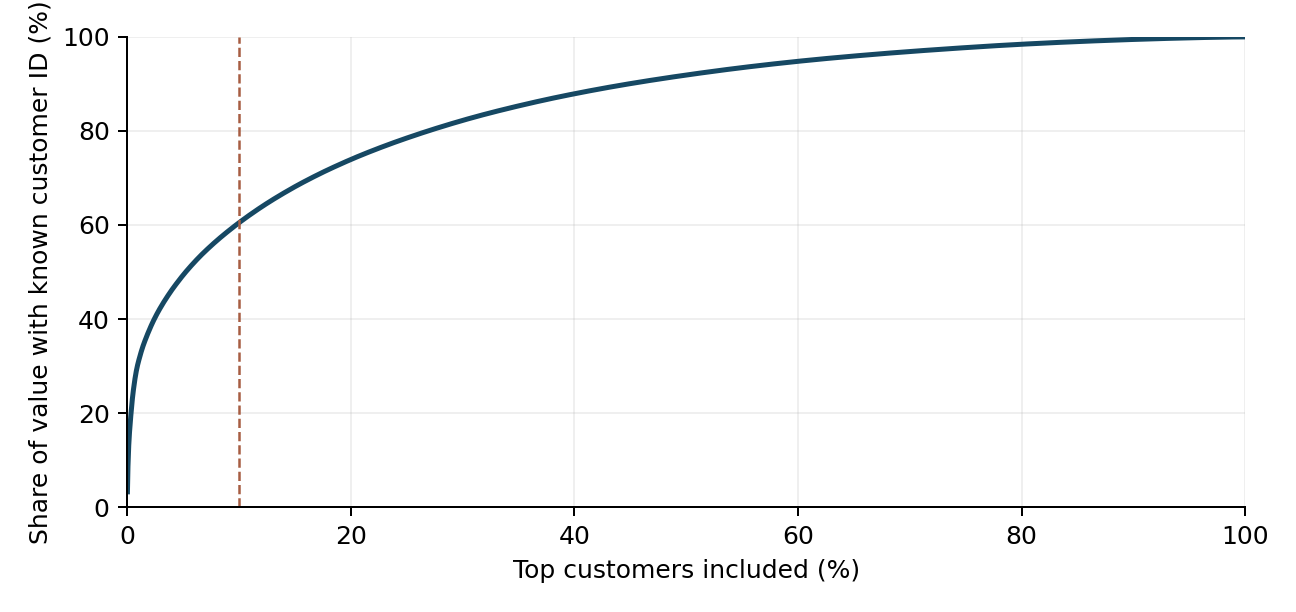
\includegraphics[width=0.72\linewidth]{customer_concentration.png}
\caption{Cumulative share of observed known-ID value, ranking customers from highest to lowest.}
\end{figure}

Among identifiable customers, the top 10\% account for 60.5\% of observed value, while the 36.1\% seen in only one eligible purchase invoice contribute 7.8\%. The former divides the 430 highest-ranked IDs' value by all known-ID eligible value; 36.1\% divides IDs by IDs, while 7.8\% divides value by value. We round the 1\% and 10\% customer cutoffs up to whole IDs (43 and 430); they are compact concentration benchmarks, not natural customer classes. An ``observed one-invoice customer'' has one distinct \emph{eligible positive purchase invoice} in this window; multiple lines in that invoice count only once, and C-coded or unpriced records do not add to the count. This is not necessarily a first-time or permanently inactive customer: purchases outside our 12-month window are unknown. Known IDs cover 85.7\% of eligible line value, so the concentration result does not describe all purchases. UCI notes that many customers are wholesalers; a large account may therefore reflect a different purchasing role rather than stronger individual consumer loyalty.\source{1} We retain the monthly series in the notebook as context: November has the highest observed value, but a single annual cycle cannot establish a recurring Christmas effect or explain its cause.

For C1 we would inspect how contribution varies with observed invoice frequency and test the concentration estimate against the largest customers, exact duplicate rows, the merchandise-code rule and missing IDs. Country comparisons would need explicit group sizes because the United Kingdom accounts for 84.6\% of total eligible value. A later ML extension could form descriptive RFM-style customer groups, provided we define an observation window and address ID coverage; this dataset does not establish future customer value. A dashboard could show a cumulative contribution curve, invoice-frequency groups and the share of value with unknown IDs.

\sectionhead{3\quad Candidate B: where cancellation records appear}
\textbf{Problem and use.} In a retrospective exercise, an operations analyst could identify periods or customer countries that merit a review of cancellation handling. Research on online retail examines cancellations, returns and stockouts as distinct operational situations, supporting the value of monitoring cancellation records.\source{3} That research does not establish the cause or financial effect of the C-coded records in our file. We call them \emph{cancellations}, following UCI, and do not relabel them as physical product returns.

\textbf{Question and measure.} In which months do C-coded merchandise invoices constitute the largest share of eligible invoices? We count C-coded lines only when quantity is negative, unit price is positive and the stock code matches the same provisional merchandise rule used for A. Requiring a positive price keeps this comparison within priced merchandise events; unpriced C-coded lines remain in the input but not the measure. We count distinct invoices, rather than lines, because the C flag identifies an invoice while its number of lines can vary. The denominator is distinct eligible positive-purchase invoices plus distinct eligible C-coded invoices in that month. This is a \emph{mix of invoice records}, not the probability that a particular purchase was cancelled later: UCI supplies no explicit original-invoice link, and the original purchase may lie outside our window.

\begin{table}[H]\centering\small
\caption{Eligible distinct invoice counts and cancellation share by month.}\label{tab:cancel}
\begin{tabular}{@{}lrrr@{}}\toprule
Month & Purchase invoices & C-coded invoices & C-coded share \\\midrule
Dec 2010 & 1,548 & 301 & 16.3\% \\
Jan 2011 & 1,080 & 247 & 18.6\% \\
Feb 2011 & 1,093 & 191 & 14.9\% \\
Mar 2011 & 1,440 & 281 & 16.3\% \\
Apr 2011 & 1,235 & 220 & 15.1\% \\
May 2011 & 1,668 & 267 & 13.8\% \\
Jun 2011 & 1,525 & 298 & 16.3\% \\
Jul 2011 & 1,451 & 235 & 13.9\% \\
Aug 2011 & 1,339 & 240 & 15.2\% \\
Sep 2011 & 1,818 & 299 & 14.1\% \\
Oct 2011 & 2,005 & 308 & 13.3\% \\
Nov 2011 & 2,751 & 396 & 12.6\% \\
\bottomrule\end{tabular}
\end{table}

\begin{figure}[H]\centering
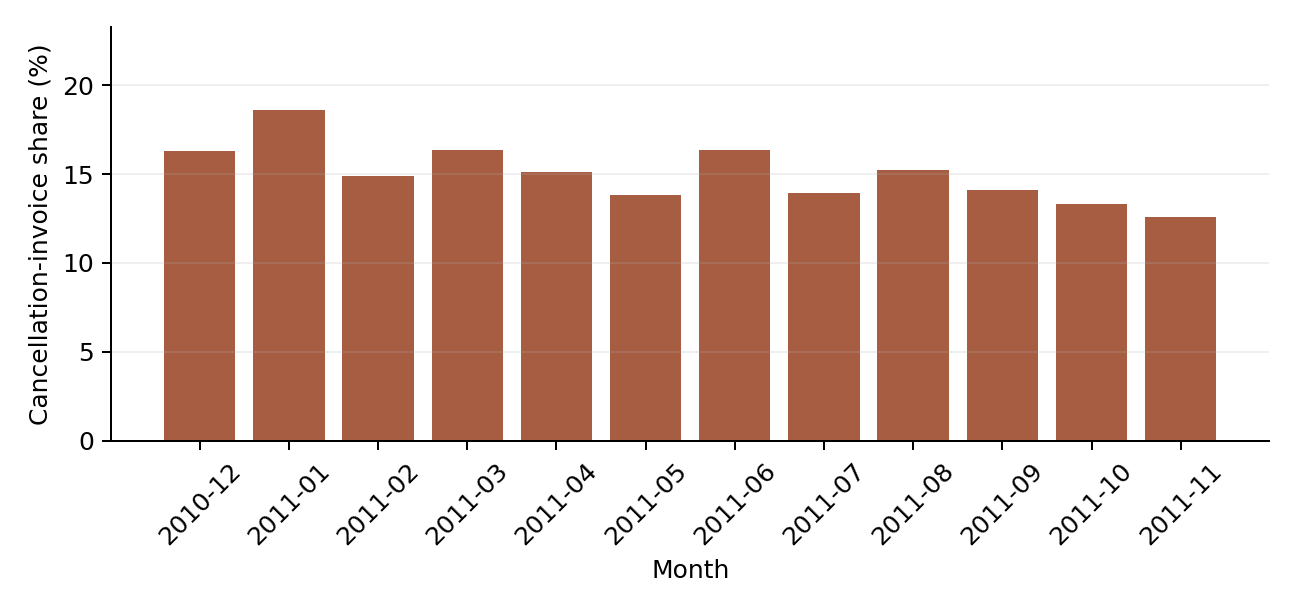
\includegraphics[width=0.72\linewidth]{monthly_cancellation_share.png}
\caption{Share of eligible distinct invoices marked C in each month.}
\end{figure}

There are \textbf{8,351 eligible cancellation lines} across \textbf{3,283 distinct C-coded invoices}. January 2011 has the highest monthly invoice share (18.6\%); November has the lowest (12.6\%). The lower November share can arise because purchase-invoice counts rose; it does not show that fewer prior purchases were cancelled or that handling improved. Each record is assigned to its own invoice month, not to the month of an original purchase. For the country comparison we switch deliberately to a \emph{line} share---eligible C-coded lines divided by eligible purchase plus C-coded lines---to indicate the mix of item-line records an operations team might review. Germany and EIRE have shares of 4.7\% and 3.7\%, respectively, versus 1.5\% for the United Kingdom. We show countries with at least 1,000 positive merchandise lines so small denominators do not dominate this first comparison; the threshold is an exploratory display rule, not a statistical guarantee, and smaller countries remain in the full table. Country represents the customer's recorded country, not a verified shipping destination. The monthly and country shares use different units and should not be compared directly; neither is a matched return or cancellation probability.

For C1, this line would require sensitivity checks for month boundaries, duplicate rows, product mix and the 1,306 negative-quantity lines without C. A useful predictive model would need a reliable original-purchase link, cancellation reasons and information available before a cancellation occurs. Without them, we would restrict later work to descriptive monitoring. An operations dashboard could show C-coded counts, eligible denominators, country/month filters and explicit data-quality flags.

\pagebreak
\sectionhead{4\quad Comparison, process framing and feedback}
\begin{table}[H]\centering\small
\caption{Distinct decisions and measurement limits of the two candidates.}
\begin{tabularx}{\linewidth}{@{}p{2.55cm}XX@{}}\toprule
 & A: customer concentration & B: cancellation records \\\midrule
Decision supported & Select customer groups for retrospective account review. & Select countries and months for process review. \\
Observed event & Positive merchandise invoice line linked by customer ID. & C-coded merchandise invoice and its lines. \\
Main strength & Invoice, customer ID and line value support contribution and frequency comparisons. & Explicit C flag makes the recorded event identifiable. \\
Main limit & Missing IDs and a bounded observation window. & No original-purchase link or reason code. \\
Future extension & RFM-style grouping after checking ID coverage. & Descriptive monitoring; prediction needs linked events. \\
\bottomrule\end{tabularx}
\end{table}

\subhead{Decision framing}
Our seven-step framing starts with a decision (customer portfolio review or process review) and a provisional success criterion: a useful comparison must state its denominator, have visible group sizes and remain interpretable under basic sensitivity checks. We use those criteria because a large difference alone may result from missing IDs, special codes or duplicate rows. The business questions are stated in Sections 2 and 3. The process is online ordering; the entities are customers, invoices, invoice lines and stock codes; the events are positive purchases and C-coded cancellations. The representation is the eight-column transaction file, and the measures are known-ID customer contribution and cancellation-record shares. The gaps become visible at the last step: the file lacks costs, promotion exposure and a purchase--cancellation key. This framing prevents a descriptive comparison from being presented as a causal explanation.

We provisionally prefer A because known-ID purchases support a clear concentration question and observable invoice frequency; we can quantify the missing-ID boundary. We would reconsider if missing-ID coverage or the largest customers made that comparison unstable, or if a reliable purchase--cancellation link made B more informative. We would ask the instructor: (1) Is a known-ID customer concentration question suitable for C1 given the 14.3\% of eligible value without an ID? (2) Is the provisional merchandise-code scope defensible despite unresolvable identical lines? (3) Would a descriptive cancellation-record question be sufficiently useful without a matched cancellation rate? Feedback is pending; no instructor response is attributed here.

\sectionhead{5\quad Measurement notes}
These counts make the analysis boundary inspectable. Each source row falls into at most one of our two eligible groups. We did not use the remaining rows to calculate purchase value or cancellation shares, and we did not delete them from the packaged input.

\begin{table}[H]\centering\small
\caption{Row flow for the 12-month case; groups are mutually exclusive.}
\begin{tabularx}{\linewidth}{@{}>{\raggedright\arraybackslash}Xr>{\raggedright\arraybackslash}X@{}}\toprule
Row group & Lines & Rule \\\midrule
All source lines in the case & 516,384 & Date within the 12 complete months. \\
Eligible positive purchase lines & 500,531 & Merchandise code; non-C invoice; positive quantity and price. \\
Eligible C-coded lines & 8,351 & Merchandise code; C invoice; negative quantity; positive price. \\
Other source lines & 7,502 & Retained in input, excluded from these two measures. \\
\bottomrule\end{tabularx}
\end{table}

\pagebreak
\subhead{Duplicate sensitivity}
The 4,989 identical rows have no line identifier that lets us distinguish a duplicate error from repeated identical items. We retained them. As a sensitivity check, removing exact duplicate rows would lower observed positive purchase-line value from \pounds9,610,990.56 to \pounds9,587,779.17, a difference of 0.24\%; the count of distinct eligible C-coded invoices remains 3,283. This small change in the \emph{overall} value does not prove that customer rankings are unchanged, because repeats could be unevenly distributed across IDs. The check bounds one aggregate effect but cannot establish which duplicate treatment is correct. The generated \texttt{case\_checks.json} and executed notebook contain the corresponding figures.

Finally, all inference is specific to a historical, unnamed UK retailer. Countries are customer countries, not verified destinations; the product codes are identifiers within this dataset, not externally validated universal product keys. Further comparison requires checking compatibility before joining another source.


\sectionhead{6\quad Process record}
\begingroup\small
\subhead{Decisions and checks}
We selected UCI Online Retail for its documented source, dictionary and licence, then checked our workbook's fields, row count and dates. We chose 12 complete months over the source's incomplete final December for monthly comparison; the extraction and counts are in \texttt{data/source\_manifest.json} and \texttt{data/case\_checks.json}. We considered November's high value as a question, but one cycle cannot establish a recurring Christmas effect. We chose customer concentration for A and kept monthly value as context (notebook, Section 2). For B, we chose invoice share because C marks an invoice and invoices contain varying numbers of lines (notebook, Section 3). We checked zero prices, stock-code exceptions and missing IDs before setting eligibility rules (Sections 1, 2 and 5; \texttt{analysis/retail\_analysis.py}). Our C1 choice remains provisional.

\subhead{Instructor feedback and response}
We had not yet received feedback on these two questions or the proposed C1 preference. Candidate A remains our provisional choice; Section 4 lists the questions on which instructor advice could change it. No response is attributed to the instructor in this version.

\subhead{Individual contributions and reflection}
We developed the overall strategy and comparison together. Mois\'{e}s concentrated on Candidate A: customer contribution, missing IDs and the November-peak interpretation (report Section 2; notebook Section 2 and \texttt{data/customer\_concentration.csv}). He learned to define the denominator before interpreting a visible pattern; his unresolved question is how much the unknown-ID purchases and largest accounts could change the concentration conclusion. Ignacia concentrated on Candidate B: C-coded invoices, invoice versus line shares and the absent original-purchase link (report Section 3; notebook Section 3 and \texttt{data/monthly\_cancellations.csv}). She learned that an identifiable cancellation record is not a purchase-level cancellation probability; her unresolved question is whether a reliable purchase link and cancellation reason could be obtained for C1. We discussed both results before making the provisional choice.

\subhead{AI use and accountability}
We used AI assistance to draft Python code and LaTeX formatting, including an explanation of row-treatment choices. We accepted the generated positive-quantity, positive-price rule only for \emph{observed priced purchase value}, after checking 2,461 zero prices and two negative-price adjustments in \texttt{data/case\_checks.json}. We revised the analysis to show missing-ID coverage and rejected a Christmas explanation for November's peak. We did not impute zero prices because that would invent charges. We ran the notebook against the packaged CSV and checked its tables and figures against this report. The questions, final rules and interpretations are ours.
\endgroup

\sectionhead{References}
\begingroup\small
\begin{enumerate}[leftmargin=1.4em,itemsep=0em,parsep=0em]
\item Chen, D. (2015). \emph{Online Retail} [dataset]. UCI Machine Learning Repository. DOI: \href{https://doi.org/10.24432/C5BW33}{10.24432/C5BW33}. Dataset and dictionary: \url{https://archive.ics.uci.edu/dataset/352/online+retail}. Accessed 25 September 2026.
\item Chen, D., Sain, S. L., \& Guo, K. (2012). ``Data mining for the online retail industry: A case study of RFM model-based customer segmentation using data mining.'' \emph{Journal of Database Marketing \& Customer Strategy Management}, 19, 197--208. DOI: \href{https://doi.org/10.1057/dbm.2012.17}{10.1057/dbm.2012.17}.
\item Son, J., Kang, J. H., \& Jang, S. (2019). ``The effects of out-of-stock, return, and cancellation amounts on the order amounts of an online retailer.'' \emph{Journal of Retailing and Consumer Services}, 51, 421--427. DOI: \href{https://doi.org/10.1016/j.jretconser.2019.02.008}{10.1016/j.jretconser.2019.02.008}. Used to motivate cancellation monitoring, not to infer financial effects from our data.
\end{enumerate}
\endgroup
\end{document}
